%\documentclass[12pt,xcolor=dvipsnames,mathserif]{beamer}
\documentclass[12pt,xcolor=dvipsnames,handout,mathserif,aspectratio=169]{beamer}

\usepackage{hyperref}

\usepackage{pgfpages}
\usepackage{colortbl}
\usepackage{multirow}
\usepackage{eurosym}

%\pgfpagesuselayout{2 on 1}[border shrink=2.5mm]
%\pgfpageslogicalpageoptions{1}{border code=\pgfusepath{stroke}}
%\pgfpageslogicalpageoptions{2}{border code=\pgfusepath{stroke}}


% Specify theme
%\usetheme{Madrid}
\usetheme{Boadilla}
% See deic.uab.es/~iblanes/beamer_gallery/index_by_theme.html for other themes

% Specify base color
%\usecolortheme[named=OliveGreen]{structure}
\usecolortheme[named=RoyalBlue]{structure}
% See http://goo.gl/p0Phn for other colors

% Specify other colors and options as required
\setbeamercolor{alerted text}{fg=Red}
\setbeamertemplate{items}[square]

% Specify some useful short commands
\newcommand{\bbl}[1]{{\color{NavyBlue} \textbf{#1}}}
\newcommand{\bre}[1]{{\color{red} \textbf{#1}}}
\newcommand{\bgr}[1]{{\color{PineGreen} \textbf{#1}}}
\newcommand{\un}{\texttt{\char`_}}
\newcommand{\tcb}{\textcolor{blue}}

\newcommand{\tc}{\textcolor}
\newcommand{\tcbl}{\textcolor{bluelight}}


% Title and author information
\title[Introductory Statistics with Excel]{Introductory Statistics with Excel}
\author[Andrew Parnell]{Andrew Parnell}
\institute[UCD]{University College Dublin \begin{center} 
\includegraphics[width=1.5cm]{UCDlogo.pdf}\end{center} }
\date[Class 5]{Class 5 - Statistical modelling and Analysis of Variance}
%\date{Lecture 2 -- part 1}

\begin{document}

\titlepage

\begin{frame}{Learning outcomes}

In this class we will cover
\begin{itemize}
\item What is a statistical model? 
\item Analysis of Variance (ANOVA)
\item 1-way ANOVA
\item 2-way ANOVA
\end{itemize}

\end{frame}

\begin{frame}{Moving from hypothesis testing to statistical modelling}

\begin{itemize}
\item Many people see statistics as just hypothesis testing and confidence intervals
\item Most academic statisticians actually work on \bbl{statistical modelling} rather than ever running hypothesis tests (confidence intervals are used by all of us)
\item A statistical model is a way of linking the data to a theoretical construct (i.e. our ideas about how the experiment worked) and to test them using statistical thinking (usually confidence intervals)
\item Most statistical models can be written as:
$$\mbox{Data} = \mbox{Structure} + \mbox{Residuals}$$
\item The \bbl{data} is what we have observed, the \bbl{structure} is a hypothesised way the experiment works, and the \bbl{residuals} are the leftover `random' variation
\end{itemize}
\end{frame}

\begin{frame}{Example: cows}

Reminder:
\begin{tabular}{ccccccc}
169.6&142&103.3&111.6&123.4&143.5&155.1\\
101.7&170.7&113.2&130.9&146.1&169.3&155.5
\end{tabular}

\begin{itemize}
\item Our statistical model might be:
$$\mbox{Data} = \mbox{Overall mean} + \mbox{Residuals}$$
\item The overall mean here might be a value that we specify (e.g. 120kg) or something we try and estimate from the data
\item The residuals need to be assigned a probability distribution, such as the normal distribution. This will have a mean (usually set to 0) and a standard deviation which again we can either specify or estimate from the data
\item For example, if we had specified that the overall mean was 120kg then our first data point would be:
$$169.6 = 120 + 49.6$$
so the residual value is 49.6. We could do this repeatedly and estimate the standard deviation from the set of residual values
\end{itemize}
\end{frame}

\begin{frame}{More complex statistical models}

\begin{itemize}
\item If we have multiple groups, e.g. the Clenbuterol data, we might have a more complicated structural part:
$$\mbox{Data} = \mbox{Mean associated with group} + \mbox{Residuals}$$
\item Depending whether the data was in e.g. run 1 or run 2, there might be a different group mean 
\item We might further decide to give different probability distributions to the residual variation in the different groups
\end{itemize}
\end{frame}

\begin{frame}{Links with $t$-tests and ANOVA}

\begin{itemize}
\item The 1-sample $t$-test (e.g. testing cow's milk yield is 120kg or not) is an example of a statistical model with one overall group mean
\item The independent samples $t$-test we met earlier is an example of a statistical model with two different group means
\item The Analysis of Variance (ANOVA) model we are about to meet is an example of a statistical model with multiple different group means (at least 2)
\end{itemize}

\end{frame}

\begin{frame}
\huge{\bbl{1-way Analysis of Variance}}
\end{frame}


\begin{frame}\frametitle{ANOVA}
\begin{center}
\bbl{ANalysis Of VAriance} is a versatile 
statistical tool for analysing how the mean value of a \textbf{quantitative response} variable is related to one or more \textbf{categorical explanatory} factors. 
\end{center}
\end{frame}


%%%%%%%%%%%%%%%%%%%%%%%%%%%%%%%%%%%%%%%%%%%%%%%%%%%
%%%%%%%%%%%%%%%%%%%%%%%%%%%%%%%%%%%%%%%%%%%%%%%%%%%
% section 3.1

\begin{frame}\frametitle{1-way ANOVA}
\emph{Example:} reduction in blood pressure.
\vspace{0.3cm}
\begin{itemize}
\item A researcher wishes to compare three different regimes for their
effectiveness in lowering blood pressure in patients diagnosed
with high blood pressure. 
\vspace{0.3cm}
\item The recommended regimes are
\begin{enumerate}
\item Medication
\item Exercise
\item Diet
\end{enumerate}
\vspace*{0.3cm}
\item Fifteen patients have volunteered to take part in the experiment.
\end{itemize}
\end{frame}


\begin{frame}\frametitle{1-way ANOVA}
\begin{itemize}
\item The BP in each patient was recorded after they had followed their recommended regime:
\vspace*{0.5cm}
\begin{center}
{\small{
\begin{tabular}{ccc} \hline
Medication& Exercise& Diet \\ \hline
10& 6& 5\\
12& 8& 9\\
9& 3& 12\\
15& 0& 8\\
13 &2& 4\\ \hline
\end{tabular}}}
\end{center}
\vspace*{0.5cm}

\item{Specific question:} \bbl{is there a difference in the mean reduction in blood pressure for the 3 regimes?}
\end{itemize}
\end{frame}


\begin{frame}
\frametitle{1-way ANOVA}
\begin{itemize}
\item  A \tc{blue}{$t$ test} is used to compare 2 population means when independent random samples are available from the populations.
\item Given 3 independent samples, $t$ tests could be used to conduct 3 tests (1 v 2, 2 v 3 and 3 v 1) but this causes problems, e.g. is the type 1 error rate still 5\%? Should the groups all have the same residual probability distribution?
\item The ANalysis Of VAriance (ANOVA) statistical model (and its associated \bbl{$F$-test}) provides a test that the means are different based on the assumption that the residual standard deviations in each group are all equal.
\end{itemize}
\end{frame}


\begin{frame}\frametitle{Experimental design}
\begin{itemize}
\item The simplest experimental design is called a \bre{completely randomised experimental design}.
\vspace{0.3cm}
\item This is an experimental design under which independent random samples of experimental units are selected for each treatment.
\vspace*{0.5cm}
\item \emph{Blood pressure example}: each patient diagnosed with high blood pressure is \tc{blue}{randomly assigned} to one of the regimes \\i.e. 5 patients in each regime.
\end{itemize}
\end{frame}

\begin{frame}\frametitle{ANOVA terminology}
\begin{itemize}
\item The \tc{blue}{response variable} is the variable being measured in the experiment:\\
\hspace*{1.9cm}\tc{red}{drop in BP}
\vspace*{0.3cm}
\item \tc{blue}{Factors} are variables applied to the object or individual in the experiment:\\
\hspace*{1.9cm}\tc{red}{regime}
\vspace*{0.3cm}
\item \tc{blue}{Factor levels} are the values of the factor used in the experiment:\\
\hspace*{1.9cm}\tc{red}{medication, exercise, diet}
\vspace*{0.3cm}
\item \tc{blue}{Treatments} are the factor-Level combinations used\\
\hspace*{1.9cm}\tc{red}{same as factor levels here!}
\vspace*{0.3cm}
\item \tc{blue}{Experimental units} are the objects on which the response variables and factor levels
are measured/recorded:\\
\hspace*{1.9cm}\tc{red}{patients}
\end{itemize}
\end{frame}

\begin{frame}\frametitle{ANOVA terminology}
\begin{itemize}
\item We are interested in assessing the \tc{blue}{the effect of the factors on the response variable}:\\
\hspace*{0.9cm}\tc{red}{effect of regime on drop in BP}
\vspace*{0.2cm}
\item \tc{blue}{Quantitative factors} are measured on a numerical scale:\\
\hspace*{0.9cm}\tc{red}{age, daily medication dose}
\vspace*{0.2cm}
\item \tc{blue}{Qualitative factors} are not measured on a numerical scale:
\hspace*{0.9cm}\tc{red}{regime}
\vspace*{0.2cm}
\item Reminder: a \tc{blue}{designed experiment} is one for which the researcher controls the specifications of the treatments and the method of assigning the experimental units to each treatment:\\
\hspace*{0.9cm}\tc{red}{completely randomized design}
\vspace*{0.2cm}
\item An \tc{blue}{observational study} is one in which the researcher simply observes the treatments and the response on a sample of experimental units:\\
\hspace*{0.9cm}\tc{red}{e.g. examine a doctor's records and record}\\
\hspace*{0.9cm}\tc{red}{regime and drop in BP for each patient}
\end{itemize}
\end{frame}

\begin{frame}
\frametitle{1-way ANOVA}
\begin{itemize}
\item In general we want to compare the means of $k$ populations.
\begin{center}
{\scriptsize{
\begin{tabular}{lccccc} \hline
& 1& 2& 3& $\ldots$& k \\ \hline
Population mean& pop mean 1 & pop mean 2 & pop mean 3 & $\ldots$& pop mean $k$ \\
Population st dev& pop sd 1 &  pop sd 2 & pop sd 3 & $\ldots$& pop sd $k$ \\
Sample size& $n_1$& $n_2$& $n_3$&$\ldots$&  $n_k$ \\
Sample mean& sample mean 1& sample mean 2 & sample mean 3 &$\ldots$&  sample mean $k$\\
Sample st dev & sample st dev 1 & sample st dev 2 & sample st dev 3 & $\ldots$& sample st dev $k$  \\ \hline
\end{tabular}}}
\end{center}
\item Formally, in ANOVA, we test:
$$H_0: \mbox{pop mean 1 = pop mean 2 = pop mean 3} = \ldots =  \mbox{pop mean } k $$
against the alternative
$$H_A: \mbox{ at least one mean is different from the others.}$$
\end{itemize}
\end{frame}


\begin{frame}\frametitle{1-way ANOVA}
\emph{Example} 
\begin{itemize}
\item For the BP experiment:\\
\vspace*{0.5cm}
\begin{center}
{\small{
\begin{tabular}{lll} \hline
Medication & Exercise & Diet\\\hline
$n_1$ = 5 & $n_2$ = 5& $n_3$ = 5 \\
$\mbox{sample mean 1}$ = 11.8 &$\mbox{sample mean 2}$ = 3.8& $\mbox{sample mean 3}$ = 7.6\\
$\mbox{sd 1}$ = 2.4& $\mbox{sd 2}$ = 3.2& $\mbox{sd 3}$ = 3.2\\
\hline
\end{tabular}}}
\end{center}
\vspace*{0.3cm}
\item Is there evidence in the data which suggests that the average BP under the 3 regimes differs?
\vspace{0.3cm}
\item Certainly the 3 sample means \emph{vary} -- but this will happen even if $H_0$ is true! 
\vspace{0.3cm}
\item Do the 3 sample means \emph{vary enough} to suggest that there is a difference in the true underlying population means?
\end{itemize}
\end{frame}

\begin{frame}\frametitle{1-way ANOVA: assumptions}
\begin{itemize}
\item Assumptions are similar to those for the 2-sample $t$-test.
\end{itemize}
\begin{enumerate}
\item The samples are independent random samples.
\vspace*{0.3cm}
\item The sample means are approximately normally distributed within each population.
\vspace*{0.3cm}
\item All populations have the \bre{same} standard deviation.
\end{enumerate}
\vspace*{0.3cm}
\end{frame}


\begin{frame}\frametitle{1-way ANOVA: assumptions}
\vspace{-0.5cm}
\begin{center}
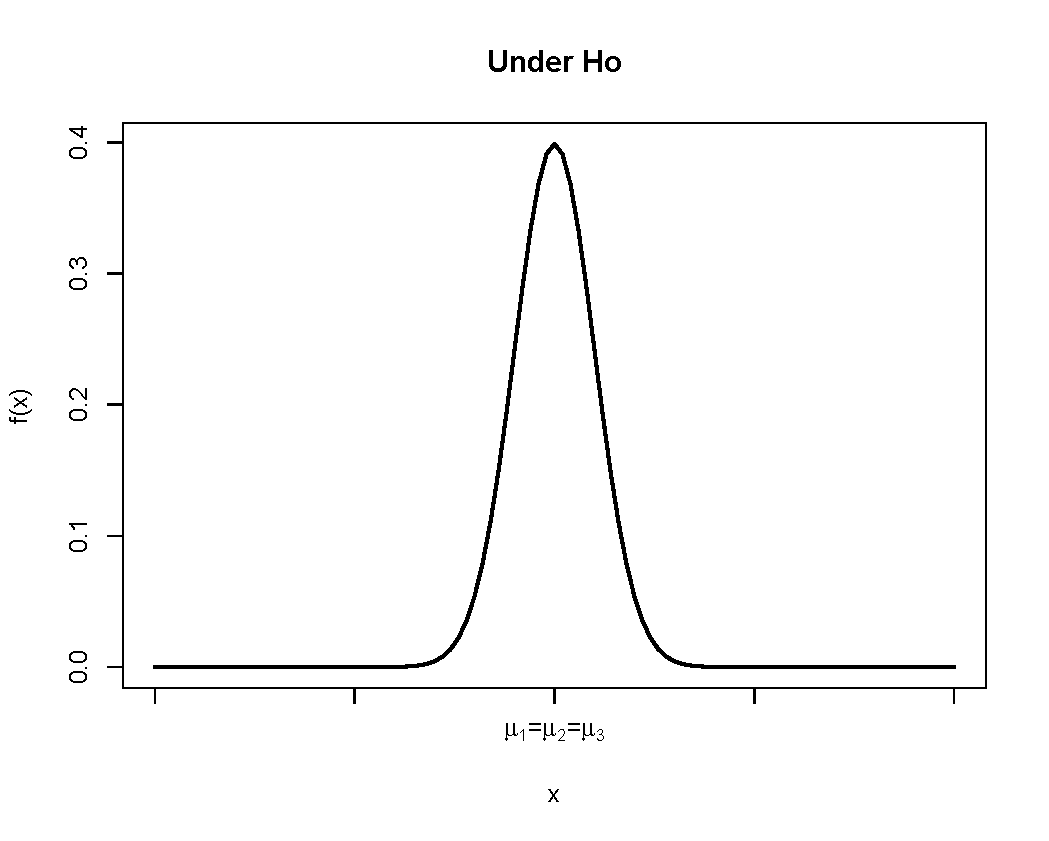
\includegraphics[width= 8cm]{UnderHoAgain.pdf}
\end{center}
\vspace{-0.5cm}
\begin{itemize}
\item Under $H_0$ all populations have the same mean.\\
Given the assumptions, all have the same residual standard deviation.
\end{itemize}
\end{frame}

\begin{frame}\frametitle{1-way ANOVA: assumptions}
\vspace{-0.5cm}
\begin{center}
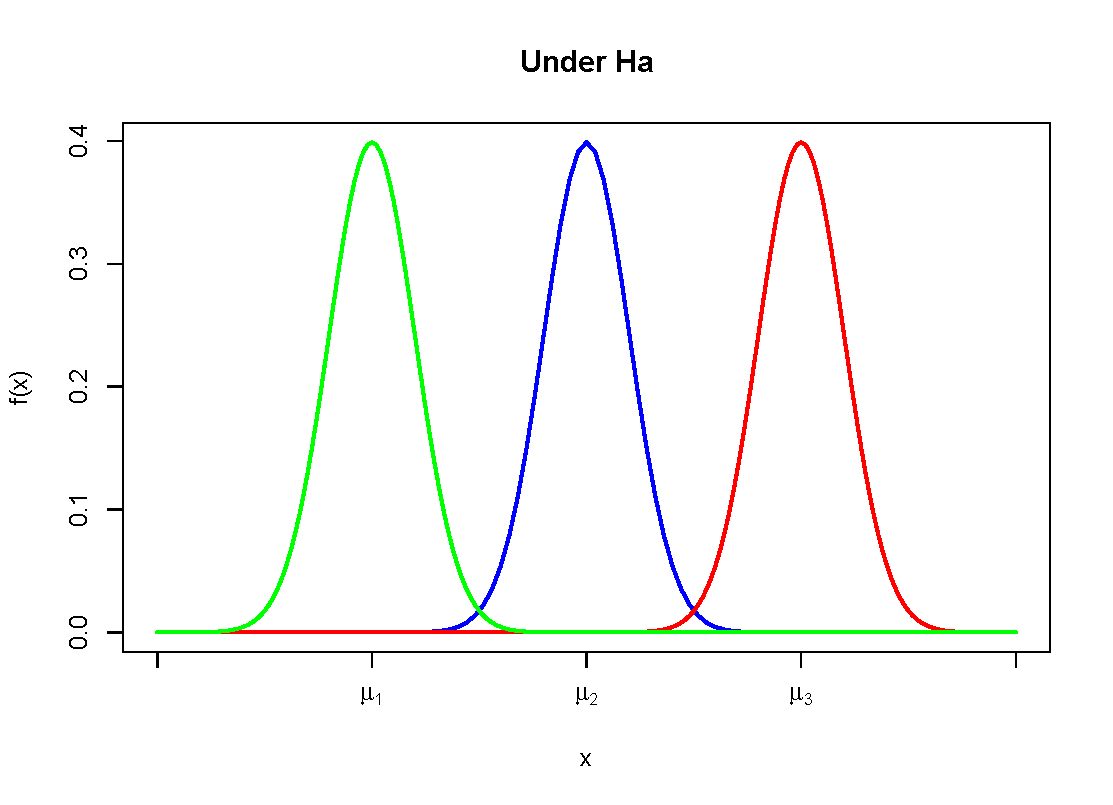
\includegraphics[width= 8cm]{UnderHa.pdf}
\end{center}
\vspace{-0.5cm}
\begin{itemize}
\item Under $H_a$ all populations have different means.\\
Given the assumptions, all have the same residual standard deviation.
\end{itemize}
\end{frame}

\begin{frame}\frametitle{1-way ANOVA}
\begin{itemize}
\item Use ANOVA to test $H_0$ (all population means equal). 
\item We do this using an \bbl{$F$-test}:
$$F = \frac{\mbox{Variation between sample means}}{\mbox{Variation within groups}}$$
\item The numerator is 0 if all means are equal -- gets larger the more spread out the means are. 
\item If that variation is `large', evidence that at least one of the means is different from the others $\Rightarrow$ reject $H_0$.
\item The denominator provides a 
guide for determining whether the numerator is `large'.
\item Comparing variation between group means to the variation within groups; hence ``analysis of variance".
\end{itemize}
\end{frame}

\begin{frame}\frametitle{1-way ANOVA}

The results are usually presented in a table with the following values:
\begin{itemize}
\item \bbl{SSTr}: the sum-of-squares associated with the treatment. This is a measure of how variable the means are between the groups
\item \bbl{SSR}: the sum-of-squares associated with the residuals. This is a measure of how variable the residuals are within a group
\item \bbl{MSTr}: the SSTr value corrected for the number of groups
\item \bbl{MSR}: the SSR value corrected for the number of observations
\end{itemize}
The ratio of these last two provides the $F$-statistic
\end{frame}

\begin{frame}{ANOVA picture}

\begin{center}
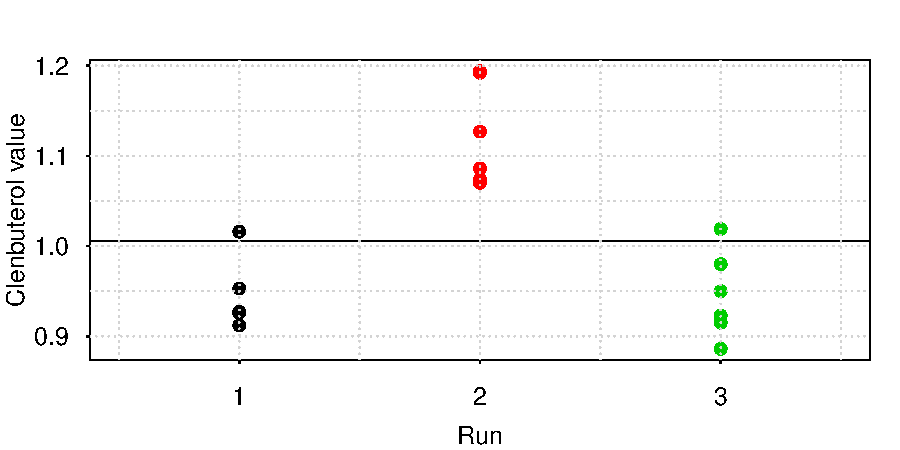
\includegraphics[width= \textwidth]{anova_plot.pdf}
\end{center}

\end{frame}

\begin{frame}\frametitle{The ANOVA table}

\vspace{0.2cm}
\begin{center}
{\small{
\begin{tabular}{lcccc}\hline
Source& df& SS& MS& F \\ \hline
&&&&\\
Treatment & $k$ - 1& SSTr& MSTr =$\displaystyle\frac{\mbox{SSTr}}{k - 1}$&$F =
 \displaystyle\frac{\mbox{MSTr}}{\mbox{MSR}}$\\
 &&&&\\
Residual &$n - k$& SSR& MSR = $\displaystyle\frac{\mbox{SSR}}{n - k}$& \\
&&&&\\
Total& $n$ - 1& SSTo&&\\
\\ \hline
\end{tabular}}}
\end{center}
SS and MS stand for sum-of-squares and mean-square respectively.
\end{frame}

\begin{frame}\frametitle{1-way ANOVA}
\begin{itemize}
\item We won't go into the details of how these values are created, but the table you get from Excel gives:
\end{itemize}
\begin{center}
{\small{
\begin{tabular}{lcccc}\hline
Source &df& SS& MS& F\\ \hline
Treatment & 2 &160.13& 80.07& 9.17\\
Residual &12& 104.80& 8.73&\\ \hline
Total &14 &264.93&&\\\hline
\end{tabular}}}
\end{center}
\vspace*{0.3cm}
\begin{itemize}
\item The residual standard deviation is obtained from $\sqrt{\mbox{MSR}} = 2.95$.
\item Excel also gives you the critical value for the F-test and the p-value, here 0.004
\item The p-value is far smaller than 0.05 so we would reject $H_0$ and conclude that, at the 5\% level there is at least one different mean
\end{itemize}
\end{frame}


\begin{frame}\frametitle{1-way ANOVA }
\emph{Example: Journal of Adolescent Research 1992} 
\vspace{0.3cm}
\begin{itemize}
\item Is musical preference associated with reckless behaviour?
\vspace{0.3cm}
\item \tc{blue}{Musical Preference:}\\
Acoustic/Pop, Mainstream Rock, Hard Rock, Heavy Metal
\vspace{0.3cm}
\item \tc{blue}{Reckless Behaviour:}\\
How many times in the past year have you indulged in reckless behaviour?
\vspace{0.3cm}
\item Here reckless behaviour is defined as `speeding over 80mph'.
\end{itemize}
\end{frame}

\begin{frame}\frametitle{1-way ANOVA}
\begin{itemize}
\item Cutting to the chase, here is the ANOVA table:\\
\begin{center}
{{
\begin{tabular}{lccccc}\hline
Source& df& SS& MS& $F$& $p$\\\hline
Treament & 3& 12.85& 4.2833& 5.09& 0.0029\\
Residual & 76& 63.9&0.8408&&\\ \hline
Total& 79& 76.75&&&\\ \hline
\end{tabular}}}
\end{center}

\item For significance level 5\% the mean number of occasions driving over 80mph differs for the groups defined in terms of musical preference.
\end{itemize}
\end{frame}

\begin{frame}
\huge{\bbl{Comparing means using ANOVA}}
\end{frame}

\begin{frame}
\frametitle{1-way ANOVA: which means differ?}
\begin{itemize}
\item If ANOVA fails to accept $H_0$ we are likely to be interested in \bgr{which} means differ.
\vspace{0.2cm}
\item To compare specific means, either with a test or confidence interval, we need the
standard error of difference \tc{blue}{SED}.
\vspace*{0.3cm}
\item For means of samples of sizes $n_1$ and $n_2$:
$$\tc{blue}{\mbox{SED} = \sqrt{\mbox{MSR}} \sqrt{\frac{1}{n_1}+\frac{1}{n_2}}}$$
\item The SED makes use of MSR to estimate the residual standard deviation, thereby using more information than a standard $t$-test between groups.
\end{itemize}
\end{frame}

\begin{frame}
\frametitle{1-way ANOVA: which means differ?}
\emph{Example: Is musical preference associated with reckless behaviour?}
\begin{itemize}
\item In this case there are 20 subjects in each treatment group, so:
$$\mbox{SED} = \sqrt{\frac{2 \times 0.84079}{20}} = 0.28996$$
\item To test at significance level 1\% with $df = 76$, the $t$ critical value (from Excel - \texttt{T.INV.2T(0.01, 73)}) is 2.642.
\item Hence, the population means differ at significance level 1\% if:
\begin{eqnarray*}
\frac{\mid\mbox{sample mean 1} - \mbox{sample mean 2} \mid}{\mbox{SED}} &>& \mbox{Critical value}\\
\end{eqnarray*}
\end{itemize}
\end{frame}

\begin{frame}
\frametitle{1-way ANOVA: which means differ?}
\begin{itemize}
\item It is useful when comparing means to define the \tc{blue}{least significant difference LSD}.
\vspace{0.3cm}
\item We define the \tc{blue}{least significant difference LSD} to be:
$$\tc{blue}{\mbox{LSD} = \mbox{Critical value} \times  \mbox{SED}}$$
\item Hence sample means 1 and 2 differ at the 1\% level if:
$$\mid\mbox{sample mean 1} - \mbox{sample mean 2} \mid >  \mbox{LSD}$$
\end{itemize}
\end{frame}

\begin{frame}
\frametitle{1-way ANOVA: which means differ?}
\emph{Example: Is musical preference associated with reckless behaviour?}
\begin{itemize}
\item We previously inferred that the means differed for the groups defined in terms of musical preference. Which means actually differ?
\vspace{0.3cm}
\begin{center}
{\small{
\begin{tabular}{ccccc}\hline
&Acoustic/& Mainstream& Hard &Heavy\\
&Pop& Rock &Rock &Metal\\ \hline
Sample means &2.50& 2.70 &2.75 &3.55\\ \hline
\end{tabular}}}
\end{center}
\vspace*{0.3cm}
\item Using a 1\% significance level
$$\mbox{LSD} =  \mbox{critical value} \times  \mbox{SED} = 2.642 \times 0.290 = 0.766 $$
\item So number of reckless events on Heavy Metal differs significantly from the others (all differences $\geq$ 0.8).
\vspace{0.3cm}
\item There are no significant differences among the other 3 groups (all differences $\leq$ 0.25).
\end{itemize}
\end{frame}

\begin{frame}\frametitle{1-way ANOVA: which means differ?}
\emph{Example: music preference/reckless behaviour.}
\begin{itemize}
\item Given that the Heavy Metal group differs significantly from the others we may wish to construct a \tc{blue}{95\% confidence interval for the mean} of the  Heavy Metal group.
\vspace*{0.3cm}
\item The mean for this group is 3.55, with standard error:
$$\sqrt{\frac{\mbox{MSR}}{20}} = \sqrt{\frac{0.841}{20}} =0.205$$
\vspace*{0.3cm}
\item The $t$ critical value, for 95\% confidence, with df = 76 is 1.992 (Excel - \texttt{T.INV.2T(0.05, 76)})
\vspace*{0.3cm}
\item Hence the CI of interest is:
$$ 3.55 \pm 1.992 \times 0.20504 = 3.55 \pm 0.4084 = (3.14, \,\,\,3.96) \mbox{ events}$$
\end{itemize}
\end{frame}

\begin{frame}
\huge{\bbl{ANOVA with randomised block designs}}
\end{frame}

\begin{frame}
\frametitle{Blocking to increase power}
\begin{itemize}
\item Power (the probability of detecting differences) is greater when there is \tc{blue}{less variation
among the experimental units}
i.e.~when the within group standard deviation is small.
\vspace*{0.1cm}
\item In such a case, most of the variation can be attributed to differences between the treatment
means and a large $F$ value is more likely.
\vspace*{0.1cm}
\item \tc{blue}{Blocking} compares values for different treatments \tc{blue}{measured on similar experimental units}.
\vspace{0.1cm}
\item \textit{Similar} means similar with respect to characteristics which influence the response.
\vspace*{0.1cm}
\item \emph{Eg:} when comparing effect of dietary regimes on weight loss, use individuals of same gender
and similar weight.
\end{itemize}
\end{frame}


\begin{frame}\frametitle{Randomised Block Design}
\begin{itemize}
\item Say we wish to conduct an experiment to compare $k$ treatment means.
\end{itemize}
\vspace*{0.3cm}
\begin{enumerate}
\item Divide the experimental units into groups of $k$ units, so that units within a group are as similar as possible.
\item Within each group randomly allocate treatments so that each unit in a group receives a
different treatment.
\end{enumerate}
\vspace*{0.3cm}
\begin{itemize}
\item The groups are called \tc{blue}{blocks}.
\vspace*{0.2cm}
\item Allocation of units to blocks is \tc{blue}{non-random}.
\vspace*{0.2cm}
\item In each block allocation of units to treatments is \tc{blue}{random}.
\end{itemize}
\end{frame}


\begin{frame}
\frametitle{Randomised block design}
\begin{itemize}
\item 40 volunteers have agreed to take part in an evaluation of 4 computer training courses.
\vspace*{0.3cm}
\item Each volunteer will be sent to one of the 4 courses and asked to complete a questionnaire at
the end of the course.
\vspace*{0.3cm}
\item From each questionnaire a general satisfaction score on a scale of 0 to 100 will be computed.
\vspace*{0.3cm}
\item Possible ways of deciding which volunteer attends which course include:
\vspace{0.2cm}
\begin{itemize}
\item completely randomised design.
\vspace{0.2cm}
\item randomised block design.
\end{itemize}
\end{itemize}
\end{frame}


\begin{frame}
\frametitle{Experimental Design}
\begin{itemize}
\item For a \tc{blue}{completely randomised design} the volunteers are listed in random order. The top
10 are sent on course 1, the next 10 on course 2, etc.
\vspace*{0.3cm}
\item For a \tc{blue}{randomised block design} the volunteers are grouped into blocks of size 4, such that members of a block are `similar'. 
\vspace{0.3cm}
\item Blocks could be constructed on the basis of the individuals previous computer experience;
the 4 most experienced in the first block, the next 4 most experienced in the next block, etc.
\vspace*{0.2cm}
\item The randomised block design could attribute part of the total variation in satisfaction
scores to the different experience levels of the volunteers. 
\vspace{0.2cm}
\item This would reduce residual variation and make it more likely that differences between the satisfaction scores for different courses
are detected as significant if they truly exist.
\end{itemize}
\end{frame}


\begin{frame}
\frametitle{Randomised block designs and ANOVA}
\emph{Example: computer course evaluation}\\
\vspace*{0.3cm}
\begin{itemize}
\item Block and Treatment Means:
\end{itemize}
\begin{center}
\vspace*{0.3cm}
{\small{
\begin{tabular}{c|cccc|c}\hline
Block& Tr 1& Tr 2& Tr 3& Tr 4& Mean\\ \hline
1& 52.1& 51.3& 57.9& 56.9& 54.550\\
2& 59.9& 58.8& 62.7& 63.4& 61.200\\
3& 63.3& 63.8& 64.3& 67.8& 64.800\\
4& 68.9& 69.3& 68.3& 74.5& 70.250\\
5& 68.5& 76.4& 75.0& 73.8& 73.425\\
6& 73.2& 80.9& 80.5& 80.1& 78.675\\
7& 83.8& 84.0& 85.6& 85.1& 84.625\\
8& 85.0& 83.4& 88.7& 91.1& 87.050\\
9& 92.8& 90.4& 91.5& 95.0& 92.425\\
10& 93.3& 95.5& 96.6& 98.8& 96.050\\ \hline
Mean &74.08& 75.38& 77.11& 78.65& 76.305\\ \hline
\end{tabular}}}
\end{center}
\end{frame}


\begin{frame}
\frametitle{Randomised block designs and ANOVA}
\begin{itemize}
\item The resulting ANOVA table is below:
\vspace*{0.3cm}
\begin{center}
{\small{
\begin{tabular}{lrrrrr}\hline
Source& DF& SS &MS & $F$ & $p$-value\\ \hline
Treatment& 3& 119.5& 39.8& \bf{10.0}& 0.0001\\
Block& 9& 6875.1& 763.9 & \bf{191.4}&$<$0.0001\\
Residual& 27& 107.8& 4.0&&\\ \hline
Corrected Total& 39& 7102.4&&&\\\hline
\end{tabular}}}
\end{center}
\vspace*{0.3cm}
\item We are not going to cover the maths of where these values come from!
\end{itemize}
\end{frame}

\begin{frame}
\frametitle{Randomised block designs and ANOVA}
\begin{itemize}
\item Conclude: there is very strong evidence ($p = 0.0001$) that mean satisfaction scores depend on the training course.
\vspace{0.2cm}
\item Conclude: block means differed significantly ($p < 0.0001$), so blocking did succeed in reducing the
residual (error) variation.
\vspace*{0.3cm}
\item \tc{blue}{Warning}: if blocking \tc{blue}{did not reduce residual error}, the randomised block design would be \tc{blue}{less powerful} that the completely randomised design.
\vspace*{0.2cm}
\item The \tc{blue}{loss of degrees of freedom} would make \tc{blue}{critical values larger}, and $F$ values would not have increased sufficiently to make up for this.
\end{itemize}
\end{frame}

%\begin{frame}\frametitle{Randomised block designs and ANOVA}
%\begin{itemize}
%\item As usual, we'll use statistical software to run ANOVA, but let's see what happens when we click `ok'.
%\vspace*{0.3cm}
%\item First, some notation:
%\end{itemize}
%\begin{center}
%{\small{
%\begin{tabular}{|l|l|}\hline
%No.~of treatments &$k$\\
%No.~of blocks &$l$\\
%No.~of experimental units& $n = k \times l$\\\hline
%\end{tabular}}}
%\end{center}
%\begin{center}
%{\small{
%\begin{tabular}{|l|l|}\hline
%Treatment Means &$\bar{x}_1, \bar{x}_2, \ldots , \bar{x}_k$\\
%Treatment Totals &$T_1, T_2, \ldots , T_k$\\
%Block Means &$\bar{b}_1, \bar{b}_2, \ldots , \bar{b}_l$\\
%Block Totals &$B_1,B_2, \ldots ,B_l$\\
%Grand Total ($T$)& $\Sigma x = \Sigma T_i = \Sigma B_j$ \\
%Grand Mean& $\bar{x} = T/n$\\\hline
%\end{tabular}}}
%\end{center}
%\begin{center}
%{\small{
%\begin{tabular}{|l|l|}\hline
%Treatment SS& $\mbox{SSTr} = l \Sigma(\bar{x}_i - \bar{x})^2$\\
%Block SS& $\mbox{SSBl} = k \Sigma (\bar{b}_j - \bar{x})^2$\\
%Total (corrected SS)& $\mbox{SSTo} =\Sigma(x - \bar{x})^2$\\\hline
%\end{tabular}}}
%\end{center}
%\end{frame}
%
%
%\begin{frame}
%\frametitle{Randomised block designs and ANOVA}
%\vspace*{0.3cm}
%\begin{center}
%{\small{
%\begin{tabular}{|l|l|} \hline
%Correction for the mean $(CM)$& $T^2/n$\\
%Treatment SS $\mbox{(SSTr)}$&$\Sigma T^2_i /l - \mbox{CM}$\\
%Treatment df &$k - 1$\\
%Block SS (SSBl)& $\Sigma B^2_j /k - \mbox{CM}$\\
%Block df &$l - 1$\\
%Total SS $\mbox{(SSTo)}$& $\Sigma x^2 - \mbox{CM}$\\
%Total df &$kl - 1$\\
%Decomposition of SSTo & $\mbox{SSTr} + \mbox{SSBl} + \mbox{SSE}$\\
%SSE& $\mbox{SSTo} -\mbox{SSTr} - \mbox{SSBl}$\\
%Residual df& $(k - 1)(l - 1)$\\ \hline
%\end{tabular}}}
%\end{center}
%\vspace*{0.3cm}
%\begin{itemize}
%\item Where does the residual df of $(k - 1)(l - 1)$ come from?
%\begin{eqnarray*}
%\nu_{resid} &=& \nu_{To} - \nu_{Tr} - \nu_{Bl}\\
%&=& (kl - 1) - (k - 1) - (l - 1)\\
%&=& kl - k - l + 1\\
%&=& (k - 1)(l - 1)\\
%\end{eqnarray*}
%\end{itemize}
%\end{frame}
%
%
%\begin{frame}
%\frametitle{Randomised block designs and ANOVA}
%\begin{itemize}
%\item For treatments and blocks define mean squares(MS) by
%$$\mbox{MS} = \frac{\mbox{SS}}{\mbox{df}}$$
%\item Then
%\begin{eqnarray*}
%F &=&\frac{\mbox{MSTr}}{\mbox{MSE}}
%\end{eqnarray*}
%with $\nu_1 = k - 1$ and $ \nu_2 = (k - 1)(l - 1)$.
%\item The hypothesis of equal treatment means will be rejected if
%$$F > F_{cv}$$
%\item $F_{cv}$ is the 100(1 - $\alpha$) percentage point of an $F$ distribution with the $\nu_1, \nu_2$ degrees of freedom.
%\vspace*{0.3cm}
%\item $p$-values are calculated as the upper tail area captured by the calculated $F$.
%\end{itemize}
%\end{frame}
%
%
%\begin{frame}\frametitle{Randomised block designs and ANOVA: DIY!}
%\emph{Example: computer training course evaluations data.}
%\vspace*{0.3cm}
%\begin{center}
%{\small{
%\begin{tabular}{c|cccc|c}\hline
%Block& Tr 1& Tr 2& Tr 3& Tr 4& Mean\\ \hline
%1& 52.1& 51.3& 57.9& 56.9& 54.550\\
%2& 59.9& 58.8& 62.7& 63.4& 61.200\\
%3& 63.3& 63.8& 64.3& 67.8& 64.800\\
%4& 68.9& 69.3& 68.3& 74.5& 70.250\\
%5& 68.5& 76.4& 75.0& 73.8& 73.425\\
%6& 73.2& 80.9& 80.5& 80.1& 78.675\\
%7& 83.8& 84.0& 85.6& 85.1& 84.625\\
%8& 85.0& 83.4& 88.7& 91.1& 87.050\\
%9& 92.8& 90.4& 91.5& 95.0& 92.425\\
%10& 93.3& 95.5& 96.6& 98.8& 96.050\\ \hline
%Mean &74.08& 75.38& 77.11& 78.65& 76.305\\ \hline
%\end{tabular}}}
%\end{center}
%\end{frame}
%
%
%\begin{frame}\frametitle{Randomised block designs and ANOVA: DIY!}
%Complete the ANOVA table by computing
%\begin{enumerate}
%\item SSTo
%\item SSTr
%\item SSBl
%\item SSE (by subraction)
%\item From these and the relevant degrees of freedom compute:
%\begin{itemize}
%\item MSTr, MSBl, MSE
%\item $F$
%\end{itemize}
%\end{enumerate}
%
%\vspace*{0.3cm}
%\begin{enumerate}
%\item[1-3:] use CM, calculated from the grand total squared $T^2$
%\item[1:] needs the sum of the squared response values, $\Sigma x^2$
%\item[2:] needs the sum of the squared treatment totals, $\Sigma T^2_i$
%\item[3:] needs the sum of the squared block totals, $\Sigma B^2_j$
%\item[4:] uses SSTo = SSTr + SSBl + SSE
%\end{enumerate}
%\end{frame}
%
%
%\begin{frame}\frametitle{Randomised block designs and ANOVA: DIY!}
%\vspace*{0.3cm}
%\hspace*{-1cm}
%{\small{
%\begin{tabular}{c|cccc|cc}\hline
%Bl& Tr 1& Tr 2& Tr 3& Tr 4& $B$ & $B^2$\\ \hline
%1& 52.1& 51.3& 57.9& 56.9& 218.2& 47611.24\\
%2& 59.9& 58.8& 62.7& 63.4& 244.8& 59927.04\\
%3& 63.3& 63.8& 64.3& 67.8& 259.2& 67184.64\\
%4& 68.9& 69.3& 68.3& 74.5& 281.0& 78961.00\\
%5& 68.5& 76.4& 75&   73.8& 293.7& 86259.69\\
%6& 73.2& 80.9& 80.5& 80.1& 314.7& 99036.09\\
%7& 83.8& 84.0& 85.6& 85.1& 338.5& 114582.25\\
%8& 85&   83.4& 88.7& 91.1& 348.2& 121243.24\\
%9& 92.8& 90.4& 91.5& 95.0& 369.7& 136678.09\\
%10& 93.3 &95.5& 96.6& 98.8& 384.2& 147609.64\\  \hline
%$T$& 740.8& 753.8& 771.1 &786.5 &3052.2& 959092.92\\ \hline
%$T^2$& 548784.64 &568214.44& 594595.21& 618582.25 &2330176.54 &\\ \hline
%\end{tabular}}}
%\vspace*{0.3cm}
%$\Sigma x^2 = 240000.54$
%\end{frame}
%%
%%\begin{frame}\frametitle{Randomised block designs and ANOVA: DIY!}
%%\begin{eqnarray*}
%%\mbox{CM} &=& T^2/n = \\
%% & &\\
%%\mbox{SSTo} &=& \Sigma x^2 - CM = \\
%%&=& \\
%% & &\\
%%\mbox{SSTr} &=& \Sigma T_{i}^{2}/l - CM = \\
%%&=& \\
%% & &\\
%%\mbox{SSBl} &=& \Sigma B_{j}^2/k- CM = \\
%%&=& 6875.109\\
%% & &\\
%%\mbox{SSE} &=& \mbox{SSTo} - \mbox{SSTr} - \mbox{SBl}\\
%%&=& \\
%%&=& 
%%\end{eqnarray*}
%%\end{frame}
%
%\begin{frame}\frametitle{Randomised block designs and ANOVA: DIY!}
%\begin{eqnarray*}
%\mbox{CM} &=& 3052.2^2/40 = 232898.121\\
% & &\\
%\mbox{SSTo} &=& 240000.54 - 232898.121\\
%&=& 7102.419\\
% & &\\
%\mbox{SSTr} &=& 2330176.54/10 - 232898.121\\
%&=& 119.533\\
% & &\\
%\mbox{SSBl} &=& 959092.92/4- 232898.121\\
%&=& 6875.109\\
% & &\\
%\mbox{SSE} &=& \mbox{SSTo} - \mbox{SSTr} - \mbox{SBl}\\
%&=& 7102.419 - 119.533 - 6875.109\\
%&=& 107.777
%\end{eqnarray*}
%\end{frame}
%
%%
%%\begin{frame}\frametitle{Randomised block designs and ANOVA: DIY!}
%%\begin{eqnarray*}
%%\mbox{MSTr} &=& SSTR/\nu_{Tr} = \\
%%&=& \\
%% & & \\
%%\mbox{MSE} &=& SSE/\nu_{resid} = \\
%%&=& \\
%% & & \\
%%F &=& MSTr/MSE = \\
%%&=& 
%%\end{eqnarray*}
%%\end{frame}
%
%
%\begin{frame}\frametitle{Randomised block designs and ANOVA: DIY!}
%\begin{eqnarray*}
%\mbox{MSTr} &=& 119.533/3\\
%&=& 39.84433\\
%\mbox{MSE} &=& 107.777/27\\
%&=& 3.991741\\
%F &=& 39.84433/3.991741\\
%&=& 9.981
%\end{eqnarray*}
%\end{frame}
%

\begin{frame}
\frametitle{Randomised block designs and ANOVA}
\begin{itemize}
\item As with a completely randomised block experiment, use a \tc{blue}{LSD} to compare particular treatment means.
\vspace{0.2cm}
\item Treatment means average $l$ values so
$$SED = \sqrt{\frac{2 \mbox{MSE}}{l}}\,\,\,\ \mbox{and as before} \,\,\,\, \mbox{LSD} = \mbox{critical value} \times \mbox{SED}.$$
\vspace{0.1cm}
\item For the training course example with 5\% significance level and critical value = =  2.052 (\texttt{T.INV.2T(0.05, 27)}):
\begin{eqnarray*}
\mbox{LSD} &=&  \mbox{critical value}\times \mbox{SED}\\
 & = & 2.052 \times \sqrt{\frac{2 \times 3.991741}{10}}\\
&=& 2.052  \times 0.8935\\
&=&  1.834\\
\end{eqnarray*}
\end{itemize}
\end{frame}


\begin{frame}\frametitle{Randomised block designs and ANOVA}
\begin{itemize}
\item The treatment means were 74.08, 75.38, 77.11 and 78.65, and the LSD is 1.834.
\item So course 3 significantly different from 1, 4 different from 1, 4 different from 2, 3 different from 2
\item 2 and 1 not significantly different from each other, similarly 3 and 2, 4 and 3 (at the 5\% significance level).
%\vspace{0.2cm}
%\item Hence means with the same underline are \textbf{not} significantly different

%\vspace*{0.5cm}
%\begin{center}
%\includegraphics[height=13cm]{LSD2.pdf}
%\end{center}
\end{itemize}
\end{frame}

\begin{frame}{Multiple comparisons}
\begin{itemize}
\item When $H_0$: all means are equal is rejected by the $F$ test
we have used the LSD (based on a $t$) test to see which means differ.
\vspace{0.2cm}
\item With $k$ = 4, for example, this involves 6 different tests: tr1 mean vs  tr2, tr1 vs tr3, etc, etc
\item When $H_0$ is true and we make many independent comparisons we will reject $H_0$ much more often than the significance level that we set (e.g. 5\%)
\item We can use a \bgr{multiple comparisons procedure} to reduce this frequency.
\item The most common is that of \bbl{Bonferroni} correction where we reduce the significance level by dividing it by the number of tests, e.g. test at the 0.05/6 = 0.83\% level instead of the 5\% level
\end{itemize}
\end{frame}

\begin{frame}
\huge{\bbl{2-way ANOVA}}
\end{frame}

\begin{frame}\frametitle{Two-way ANOVA}
\begin{itemize}
\item Two-way ANOVA examines the effect of 2 categorical factors on the mean of a quantitative response variable.
\end{itemize}
\vspace*{0.5cm}
\textbf{Examples}
\begin{itemize}
\item effect of \tc{blue}{variety} (3 levels) and \tc{blue}{planting density} (10, 20, 30 thousand plants per hectare) on \tc{blue}{yield} of tomato plants.
\vspace{0.5cm}
\item effect of investment \tc{blue}{manager} (3 levels) and \tc{blue}{investment type} (4 levels) on \tc{blue}{5 year yield} on a \euro 10,000 investment.
\item Effect of 
\end{itemize}
\end{frame}

\begin{frame}
\frametitle{Factorial experimental designs}
\begin{itemize}
\item Effect of two or more treatments explored simultaneously.
\vspace{0.3cm}
\item Every level of each treatment is studied under the conditions of every level of all other treatments.
\vspace{0.3cm}
\item Two, three, four, $\ldots$, $n$ treatments can be studied in same experiment.
\vspace{0.3cm}
\item Here we'll consider only 2.
\end{itemize}
\end{frame}

\begin{frame}
\frametitle{Advantages of factorial experimental designs}
\begin{itemize}
\vspace{0.3cm}
\item Need 2 completely randomised designs to analyse effects of two treatments.
\vspace{0.3cm}
\item Factorial design can analyse the effect of 2 treatments together, saving time and effort.
\vspace{0.3cm}
\item Can be use to control confounding variables, by building such variables into the experimental design.
\vspace{0.3cm}
\item Increased power: effects of second variable removed from the SSR.
\vspace{0.3cm}
\item Perhaps most importantly: can explore possible interaction between two treatment variables.
\end{itemize}
\end{frame}

\begin{frame}
\frametitle{Factorial experimental designs: example}
\begin{itemize}
\item  The time required to make coke from coal was examined in a $2 \times 3$ experiment with $18$ observations.
\item The effect of oven width and oven temperature on the process are of interest.
\item Oven width has three levels: 4, 8 and 12 inches.
\item Oven temperature has two levels: 1600$^o$F and 1900$^o$F.
\end{itemize}
\small
\begin{center}
\begin{tabular}{ccc}\hline
width	&temp	&time\\\hline
4	&1600	&3.5\\
4	&1600	&3.0\\
4	&1600	&2.7\\\hline
4	&1900	&2.2\\
4	&1900	&2.3\\
4	&1900	&2.4\\\hline
8	&1600	&7.1\\
$\vdots$ &$\vdots$	&$\vdots$\\
\end{tabular}
\end{center}
\end{frame}

\begin{frame}
\frametitle{Factorial experimental designs: example}
\begin{itemize}
\item  The intersection of each level of each treatment gives rise to \textbf{cells}: in the example, there are 3 observations in each of 6 cells.
\vspace{0.3cm}
\item One treatment is arbitrarily designated the \textbf{row treatment}: here let's make the the oven width.
\vspace{0.3cm}
\item The other treatment is the \textbf{column treatment}: here that's oven temperature.
\vspace{0.3cm}
\item For this module, only consider designs with equal numbers of observations in each cell.
\end{itemize}
\end{frame}

\begin{frame}
\frametitle{Two-way ANOVA}
\begin{itemize}
\item Factorial designs with 2 factors are analysed using a two-way ANOVA.
\vspace{0.2cm}
\item Two-way ANOVA tests the following hypotheses:
\end{itemize}
\begin{center}
\begin{tabular}{lcl}
Row effects: & $H_0:$ & Row means are all equal.\\
                       & $H_A:$ & At least one row mean is different.\\
                        & & \\
Column effects: & $H_0:$ & Column means are all equal.\\
                       & $H_A:$ & At least one column mean is different.\\
                        & & \\
Interaction effects: & $H_0:$ & The interaction effects are 0.\\
                       & $H_A:$ & An interaction effect is present.\\
\end{tabular}
\end{center}
\end{frame}


\begin{frame}
\frametitle{Two-way ANOVA: main effects and interactions}
\begin{itemize}
\item The row effects and column effects are often called \tc{blue}{main effects}.
\vspace{0.3cm}
\item Essentially effect = mean difference between levels.
\vspace{0.3cm}
\item An \tc{blue}{interaction} occurs when the effect of one treatment varies according to the levels of the other treatment.
\vspace{0.3cm}
\item In a factorial design, interaction occurs when the pattern of cell means in one row (going across the columns) varies from the cell mean pattern in another row.
\vspace{0.3cm}
\item Similarly, interaction occurs when the pattern of cell means differs between columns.
\end{itemize}
\end{frame}

\begin{frame}
\frametitle{Graphically depicting interactions}
\begin{itemize}
\item Denote the no. of levels in the row treatment by $R$, and similarly in the column treatment by $C$.
\vspace{0.2cm}
\item In the coking experiment $R=3$ and $C=2$.
\vspace{0.2cm}
\item Can graphically examine factorial design experiment data by plotting cell means within each row (say) and connecting them with a line.
\vspace{0.2cm}
\item If the $R$ lines are parallel, no interaction is indicated.
\end{itemize}
\end{frame}

\begin{frame}
\frametitle{Graphically depicting interactions}
\begin{center}
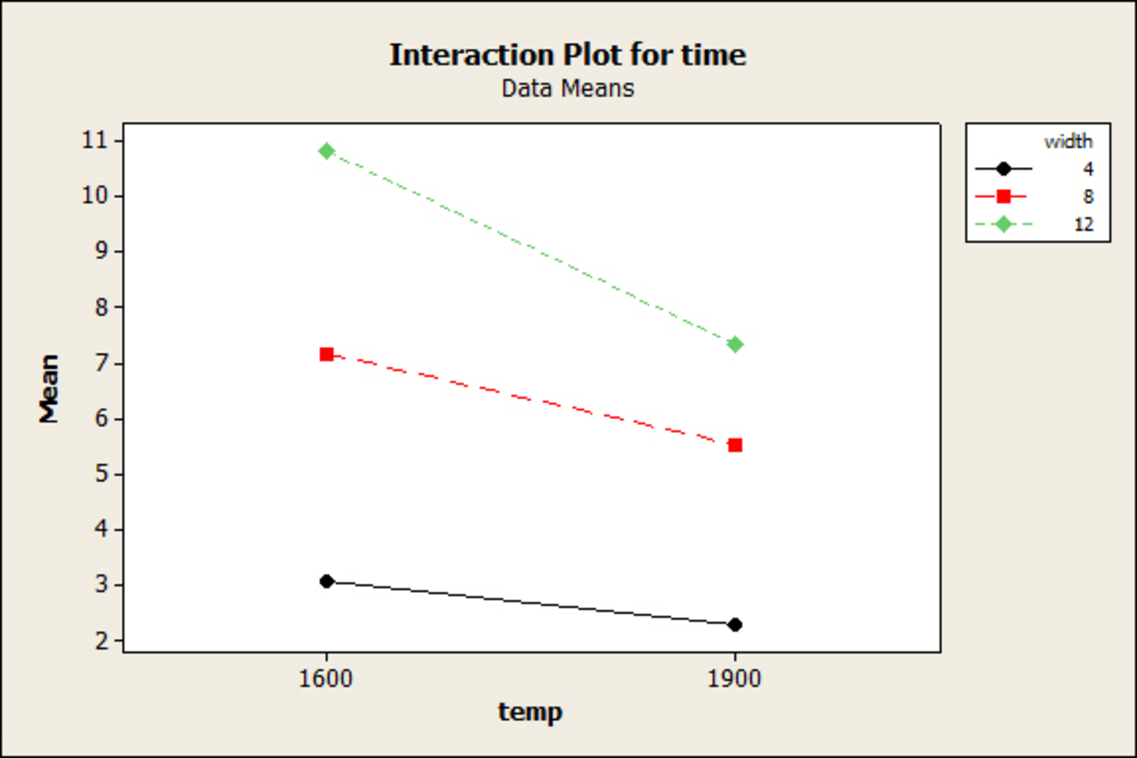
\includegraphics[width=8cm]{Interaction.pdf}
\end{center}
\begin{itemize}
\item If the lines are parallel there is likely to be no interaction. Looks like there might be interaction here.
\end{itemize}
\end{frame}

\begin{frame}
\frametitle{Interpreting effects in the presence of interaction}
\begin{itemize}
\item When interaction effects are significant, main effects are confounded and \textbf{should not be analysed in the usual manner}.
\vspace{0.2cm}
\item It is not possible in such a case to state that row or column effects are significant as the main effect of one treatment varies with the levels of the other main effect.
\end{itemize}
\end{frame}

\begin{frame}
\frametitle{Two-way ANOVA table: coking example.}
\begin{center}
		\begin{tabular}{lcl}
		Width effect: & $H_0:$ & Row means are all equal.\\
		                       & $H_A:$ & At least one row mean is different.\\
		                        & & \\
		Temp. effects: & $H_0:$ & Column means are all equal.\\
		                       & $H_A:$ & At least one column mean is different.\\
		                       & & \\
		Interaction effects: & $H_0:$ & The interaction effects are 0.\\
		                       & $H_A:$ & An interaction effect is present.\\
		\end{tabular}
		\end{center}
\begin{itemize}
\item To test these three hypotheses we, as usual, determine a $F$ test statistic for each.
\end{itemize}
\end{frame}

%\begin{frame}
%\frametitle{Two-way ANOVA table: notation.}
%\begin{itemize}
%\item $n$ = no. of observations in a cell ($n = 3$).
%\vspace{0.1cm}
%\item $i = 1, \ldots, R$ denotes row (width) treatment levels.
%\vspace{0.1cm}
%\item $j = 1, \ldots, C$ denotes column (temp) treatment levels.
%\vspace{0.1cm}
%\item $k = 1, \ldots, n$ denotes cell member.
%\vspace{0.1cm}
%\item $x_{ijk} = $ individual observation (time).
%\vspace{0.1cm}
%\item $\bar{x}_{ij} = $ cell mean.
%\vspace{0.1cm}
%\item $\bar{x}_{i} = $ row mean.
%\vspace{0.1cm}
%\item $\bar{x}_{j} = $ column mean.
%\vspace{0.1cm}
%\item $\bar{x} = $ grand mean.
%\end{itemize}
%\end{frame}
%
%
%\begin{frame}
%\frametitle{Decomposing SSTo}
%\begin{itemize}
%\item For a row factor with $R$ levels and a column factor with $C$ levels the decomposition of the total sum of squares is:
%\end{itemize}
%\begin{center}
%SSTo = SSR + SSC + SSI + SSE
%\end{center}
%\begin{center}
%\vspace*{0.5cm}
%{\small{
%\begin{tabular}{lcc} \hline
%Source of variation& SS& df\\ \hline
%Row factor & SSR& $R$ - 1\\
%Column factor& SSC& $C$ - 1\\
%Interaction& SSI& ($R$ - 1)($C$ - 1)\\
%Residual& SSE& $RC(n$ - 1)\\ \hline
%\end{tabular}}}
%\end{center}
%\vspace*{0.5cm}
%\textbf{Note that:}\\
%\begin{center}
%SSE = SSTo - SSR - SSC - SSI\\
%$RC(n$ - 1) = ($RCn$ - 1) - ($R$ - 1) - ($C$ - 1) - ($R$ - 1)($C$ - 1)
%\end{center}
%\end{frame}
%
%\begin{frame}
%\frametitle{Computing a two-way ANOVA table}
%\begin{itemize}
%\item SST: each observation from grand mean:
%$$\tc{blue}{\mbox{SST } = \Sigma \Sigma \Sigma (x_{ijk} - \bar{x})^2}$$ 
%\item SSE: each value from its cell mean:
%$$\tc{blue}{\mbox{SSE } = \Sigma \Sigma \Sigma (x_{ijk} - \bar{x}_{ij})^2}$$
%\item SSR: each row mean from the grand mean:
%$$\tc{blue}{\mbox{SSR } = nC \Sigma (\bar{x}_i - \bar{x})^2}$$ 
%\item SSC: each column mean from the grand mean:
%$$\tc{blue}{\mbox{SSC } = nR \Sigma (\bar{x}_j - \bar{x})^2}$$
%\item SSI: each cell mean from the row, column and grand means:
%$$\tc{blue}{\mbox{SSI } = n \Sigma \Sigma (\bar{x}_{ij} - \bar{x}_{i} - \bar{x}_{j} - \bar{x})^2}$$
%\end{itemize}
%\end{frame}


\begin{frame}
\frametitle{Computing a two-way ANOVA table}
\begin{center}
\begin{tabular}{lccccc} \hline
\textbf{Source}     &  \textbf{df} &      \textbf{SS}   &    \textbf{MS}   &    $\mathbf{F}$ &     $\mathbf{p}$\\\hline
  &&&&&\\
 Row factor & $Ro - 1$  & SSRo &  $\frac{\mbox{SSRo}}{Ro - 1}$ &  $\frac{\mbox{MSRo}}{\mbox{MSR}}$  &  \\
  &&&&&\\
Column factor & $C - 1$ &  SSC &$\frac{\mbox{SSC}}{C - 1}$ &  $\frac{\mbox{MSC}}{\mbox{MSR}}$  &  \\
  &&&&&\\
Interaction  & $(Ro - 1)\times (C - 1)$ & SSI & $\frac{\mbox{SSI}}{(Ro - 1)\times (C - 1)}$ &  $\frac{\mbox{MSI}}{\mbox{MSR}}$  &  \\
  &&&&&\\
Residual      &  $Ro \times \times C\times (n - 1)$  &  SSR & $\frac{\mbox{SSE}}{Ro \times C\times (n - 1)}$ &    &  \\\hline
Total      &  $Ro \times  Cn - 1$ &  SST & & & \\\hline
\end{tabular}
\end{center}
\end{frame}


\begin{frame}
\frametitle{Two-way ANOVA: coking example.}
\begin{center}
\begin{tabular}{lrrrrr} \hline
Source    &   DF &      SS  &     MS  &     F &     P\\\hline
width      &   2 & 123.1  &61.6  &222.1  & $<$0.001\\
temp        &  1   &17.2  &17.2  & 62.1  & $<$0.001\\
Interaction &  2   & 5.7  & 2.9   &10.3  &0.003\\
Error       & 12   & 3.3  & 0.3 &&\\\hline
Total      &  17 & 149.4 &&&\\\hline
\end{tabular}
\end{center}
\vspace*{0.5cm}
\begin{itemize}
\item First, test for interaction:
$$F = \frac{\mbox{MSI}}{\mbox{MSE}}  = \frac{2.8506}{0.2772} = 10.28$$
\item At the 5\% level, the critical value is 3.885 (\texttt{F.INV(0.95, 2, 12)}).
\vspace{0.2cm}
\item Hence, there is very strong evidence of a width $\times$ temperature interaction -- the `no interaction' null hypothesis is rejected at the 5\% level.
\end{itemize}
\end{frame}


\begin{frame}
\frametitle{Two-way ANOVA: coking example.}
\begin{itemize}
\item So, the interaction term is significant. Looking at the cell means gives us an idea of what's happening:
\vspace{0.2cm}
\begin{center}
\begin{tabular}{cc|cc}
& & \multicolumn{2}{c}{Temp}\\
  &  &    1600  &   1900\\\hline
&4  & 3.07 & 2.30\\
Width &8   &7.17 & 5.53\\
&12 &10.80 & 7.33\\\hline
\end{tabular}
\end{center}
\vspace{0.2cm}
\item The difference in time to coking at high and low temperatures increases with oven width.
\vspace{0.2cm}
\item \textbf{When this is the case the individual tests for the two factors make no sense.}
\end{itemize}
\end{frame}


\begin{frame}
\frametitle{Two-way ANOVA: tests following a significant interaction}
\begin{itemize}
\item In the case of a significant interaction, we can compare temperatures at each width, using an \tc{blue}{LSD}.
\vspace{0.2cm}
\item Each cell mean is calculated from $n  = 3$ observations so
\begin{eqnarray*}
\mbox{SED}  = \sqrt{\frac{2\mbox{MSR}}{n}}
 & = & \sqrt{\frac{2 \times 0.2772}{3}} \\
&=& 0.4298837\\
\mbox{critical value} &=& 2.179\\ \\
\mbox{Therefore LSD} &=& (2.179)\times(0.4298837)\\
&=&  0.937
\end{eqnarray*}
\item Only the means at width 4 under both temperatures are not significantly different, at the 5\% level.
\end{itemize}
\end{frame}

\begin{frame}
\frametitle{Two-way ANOVA: example 2} 
\begin{itemize}
\item A study on how zooplankton live in 2 lakes. 
\item 12 tanks have been set up: 6 with water from Lake Rose, and 6 with water from Lake Dennison. 
\item One of three nutrient supplements to each tank.
\item After 30 days, count the zooplankton in unit volume of water.  
\item Use two-way ANOVA to test if the population means are equal, or equivalently, to test whether there is significant evidence of interactions and main effects.
\end{itemize}
\begin{center}
\begin{tabular}{ccl}\hline
Zooplankton	&Supplement	&Lake\\\hline
34	&1&	Rose\\
43	&1	&Rose\\
57	&1	&Dennison\\
40	&1	&Dennison\\
85	&2	&Rose\\
$\vdots$	&$\vdots$	&$\vdots$\\
\end{tabular}
\end{center}
\end{frame}


\begin{frame}
\frametitle{Two-way ANOVA: zooplankton example}
\begin{center}
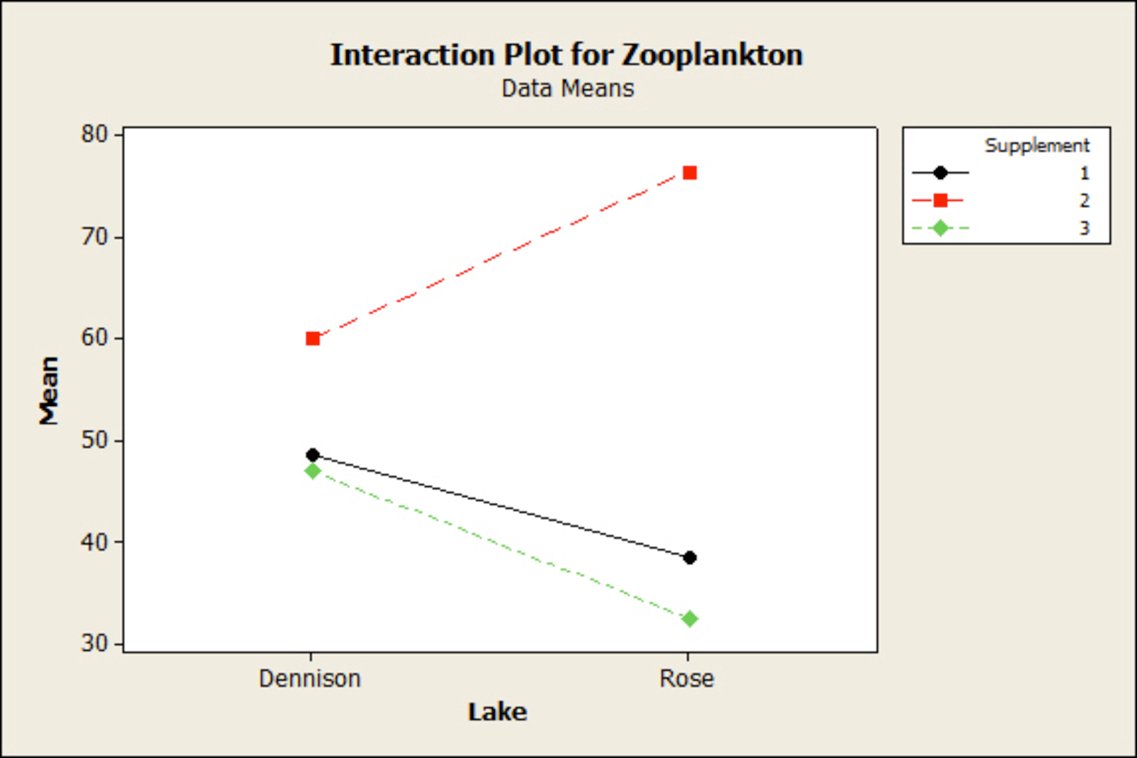
\includegraphics[width=8cm]{InteractionPlotforZooplankton.pdf}
\end{center}
\end{frame}

\begin{frame}
\frametitle{Two-way ANOVA: zooplankton example}
\vspace*{0.5cm}
\begin{center}
{\small{
\begin{tabular}{lrrrrr} \hline
Source& df& SS& MS& $F$& $p$\\ \hline
Supplement    &2  &1918.50  &959.25  &9.25  &0.015\\
Lake          &1    &21.33   &21.33  &0.21 & 0.666\\
Interaction   &2   &561.17  &280.58 & 2.71&  0.145\\
Residual         &6   &622.00  &103.67 & & \\\hline
Total        &11  &3123.00 & & &\\\hline
\end{tabular}}}
\end{center}
\vspace*{0.5cm}
\begin{itemize}
\item \underline{Test for interaction:} $p = 0.145$
\vspace*{0.3cm}
\item There is no significant evidence for a supplement$\times$lake interaction at the 5\% level
\vspace*{0.3cm}
\item i.e.~the effect of supplement is the same for the two lakes.
\end{itemize}
\end{frame}


\begin{frame}
\frametitle{Two-way ANOVA: zooplankton example}
\begin{itemize}
\item Since the interaction is  not significant we regard it as random error and combine it with SSE.
\vspace*{0.3cm}
\item Therefore, we also add the interaction df to the error df.
\vspace*{0.3cm}
\item Therefore need to re-compute all the relevant MS,  $F$ test statistics and $p$ values.
\begin{center}
\begin{tabular}{lccccc} \hline
Source& df& SS& MS& $F$& $p$\\ \hline
Supplement    &2  &1918.50  &959.250  &6.49  &0.021\\
Lake          &1    &21.33   &21.333  &0.14 & 0.714\\
Residual         &8   &1183.17  &147.8963 & & \\\hline
Total        &11  &3123.00 & & &\\\hline
\end{tabular}
\end{center}
\vspace*{0.3cm}
\item At 5\% level: significant supplement effect, but no significant lake effect.
\end{itemize}
\end{frame}


%\begin{frame}
%\frametitle{Two-way ANOVA: zooplankton example}
%\begin{itemize}
%\item We know the differences between the two lakes are the same for all supplement types.
%\vspace{0.2cm}
%\item We know there are significant differences between supplements ($p = 0.021$).
%\vspace{0.2cm}
%\item We can estimate differences between any two supplements by subtracting overall supplement means.
%\vspace{0.5cm}
%\begin{center}
%\begin{tabular}{l|ccc} \hline
%Supplement& 1& 2& 3\\ \hline
%Mean&  43.50  & 68.25  &   39.75 \\ \hline
%\end{tabular}
%\end{center}
%\end{itemize}
%\end{frame}

\begin{frame}
\frametitle{Two-way ANOVA: zooplankton example}
\begin{center}
\begin{tabular}{l|ccc} \hline
Supplement& 1& 2& 3\\ \hline
Mean&  43.50  & 68.25  &   39.75 \\ \hline
\end{tabular}
\end{center}
\begin{itemize}
\item Each mean is based on 4 values (2 tanks from each lake) so:
\begin{eqnarray*}
\mbox{SED} &=& \sqrt{\frac{2\mbox{MSR}}{4}} = \sqrt{\frac{2 \times147.896 }{4}}\\
&=& 8.599\\ \\
\mbox{Since}\,\, \mbox{critical value} &=& 2.306\\
\mbox{LSD} &=& 2.306 \times 8.599 = 19.83\\
\end{eqnarray*}
\item The means under both supplement 1 and supplement 3 differ significantly from the mean zooplankton count under supplement 2.
\end{itemize}
\end{frame}

%
%\begin{frame}\frametitle{Two-way ANOVA: zooplankton example}
%\tc{blue}{Exercise: find a 95\% confidence interval for the
%difference between the means under supplement 1 and supplement 2.}\\
%$\:$\\
%\vspace{0.2cm}
%\tc{blue}{\textbf{Steps of Solution}}
%\begin{itemize}
%\item Find the overall supplements means (43.50 and 68.25 here).
%\vspace*{0.3cm}
%\item Calculate the difference.
%\vspace*{0.3cm}
%\item Calculate SED = $\sqrt{2\mbox{MSE}/n}$ where $n$ is the number of
%observations involved in each mean.
%\vspace*{0.3cm}
%\item CI is of form
%$$\mbox{difference} \pm t_{cv} \mbox{SED}$$
%where the critical value depends on the confidence level and
%the df involved in estimating $\sigma$, i.e.~the error df.
%\end{itemize}
%\end{frame}
%
%
%\begin{frame}
%\frametitle{Section 4.5: Summary sheet 1}
%\begin{itemize}
%\item When there is no significant interaction, regard the SSI as random error and combine it with the SSE.
%\vspace{0.2cm}
%\item Accordingly, need to update the error df, and the MS, $F$ and $p$ values in the ANOVA table for the main effects.
%\vspace{0.2cm}
%\item In the presence of significant main effects, examine differences in the means at each level of the relevant factor, and use LSD or CIs to see where the differences lie.
%\end{itemize}
%\end{frame}

\begin{frame}{Summary of class 5}

\begin{itemize}
\item These are all examples of \bgr{statistical models}, either with a single mean, or a set of means for each group / treatment / block
\item In general ANOVA models assume that all the residuals have the \bre{same} standard deviation
\item We run \bbl{$F$-tests} to determine whether the overall means are different, then LSD tests (possibly with multiple comparisons correction) to determine which means are \bgr{different}
\item We can use 1-way, 2-way, etc, ANOVA to test for \bgr{multiple effects and their interactions}
\end{itemize}
\end{frame}



\end{document}
